\section{Alcance y objetivos}
Antes de iniciar el desarrollo de un proyecto, resulta imprescindible definir con claridad el objetivo 
principal que se desea alcanzar, descomponiéndolo en subobjetivos que permitan planificar de 
manera estructurada las tareas a abordar en cada una de las fases que contiene el ciclo de vida 
del proyecto.

En esta sección se establece el objetivo general del trabajo y se delimita su alcance, describiendo 
además los principales artefactos generados a lo largo del proceso de desarrollo.
\subsection{Objetivos}

Los principales \textbf{objetivos} que se abordan con este proyecto son los siguientes:
\begin{enumerate}[label=\arabic*.]
    \item Adquirir conocimientos básicos sobre la creación y edición de vídeo 
    mediante el uso de las herramientas más demandadas actualmente en el sector.
    \item Analizar y comparar distintas herramientas de edición de vídeo, 
    identificando sus ventajas, desventajas y casos de uso específicos.
    \item Desarrollar en el lector la capacidad de pensamiento crítico 
    en la selección de herramientas según los objetivos de su proyecto.
    \item Aplicar los conocimientos adquiridos mediante la creación y edición 
    de un tráiler de vídeo.
    \item Elaborar recursos educativos complementarios 
    (actividades, tutoriales, podcast, infografías) que refuercen 
    los conocimientos adquiridos durante todo el proyecto.
\end{enumerate}

\subsection{Alcance}

El alcance del presente proyecto se limita al estudio de diferentes herramientas 
demandadas actualmente en el sector orientadas a la creación y edición de vídeos, 
aplicadas a un caso práctico, como es el desarrollo de un tráiler de vídeo.

El proyecto se centra exclusivamente a la fase de 
\textbf{planificación, creación, edición y postproducción}, 
aplicando metodologías, técnicas y herramientas digitales sin abordar aspectos avanzados 
de grabación profesional, producción cinematográfica ni maquetación, modelado y animación 3D.\\
Como resultado del proyecto, se generarán los siguientes artefactos:
\begin{itemize}
    \item Un tráiler de vídeo, creado y editado por las herramientas indicadas 
    en el presente documento.
    \item Un vídeo que cuenta con un tutorial sobre el tráiler de vídeo creado, 
    indicando al detalle las herramientas y técnicas utilizadas, así como, cómo se han utilizado.
    \item Un podcast donde los autores presentan, detallan y contextualizan el proyecto, 
    haciendo principal hincapié en los problemas que se han encontrado durante el proceso 
    de desarrollo.
    \item Una infografía que resume el contenido del proyecto apoyándose de frases 
    cortas y elementos visuales, además de resaltar las ideas clave de este.
\end{itemize}

El alcance temporal toma como referencia el horario de planificación estipulado 
en la asignatura Procesamiento de la Información Multimedia. 
Todas las actividades y artefactos generados han sido realizadas dentro del tiempo 
disponible durante dicho periodo.

Como constancia de la planificación relacionada con el alcance temporal (véase la Figura~\ref{fig:tareas-gantt}, Figura~\ref{fig:diagrama-gantt}). Representa 
un \textbf{diagrama de Gantt}, donde de manera visual se recogen las tareas o artefactos temporales 
a realizar por los autores del presente proyecto. De esta manera se estipularon fechas de elaboración 
asociadas a las diferentes tareas para mantener un orden de desarrollo.

Su leyenda es fácil de comprender, los rectángulos verdes hacen referencia a tareas ya \textbf{completadas y finalizadas} 
en tiempo. Paralelamente, los rectángulos morados hacen referencia a tareas \textbf{en curso}.

Respecto al software utilizado para la configuración del diagrama, se ha hecho uso de una potente 
herramienta de planificación en entornos empresariales muy novedosa, llamada \textbf{ClipCut} 
(Más información sobre esta herramienta).

\begin{figure}[H]
    \centering
    \includegraphics[width=0.4\textwidth]{assets/actividades-gantt.png}
    \caption{Tareas configuradas en el \textbf{diagrama de Gantt}}
    \label{fig:tareas-gantt}
\end{figure}

\begin{figure}[H]
    \centering
    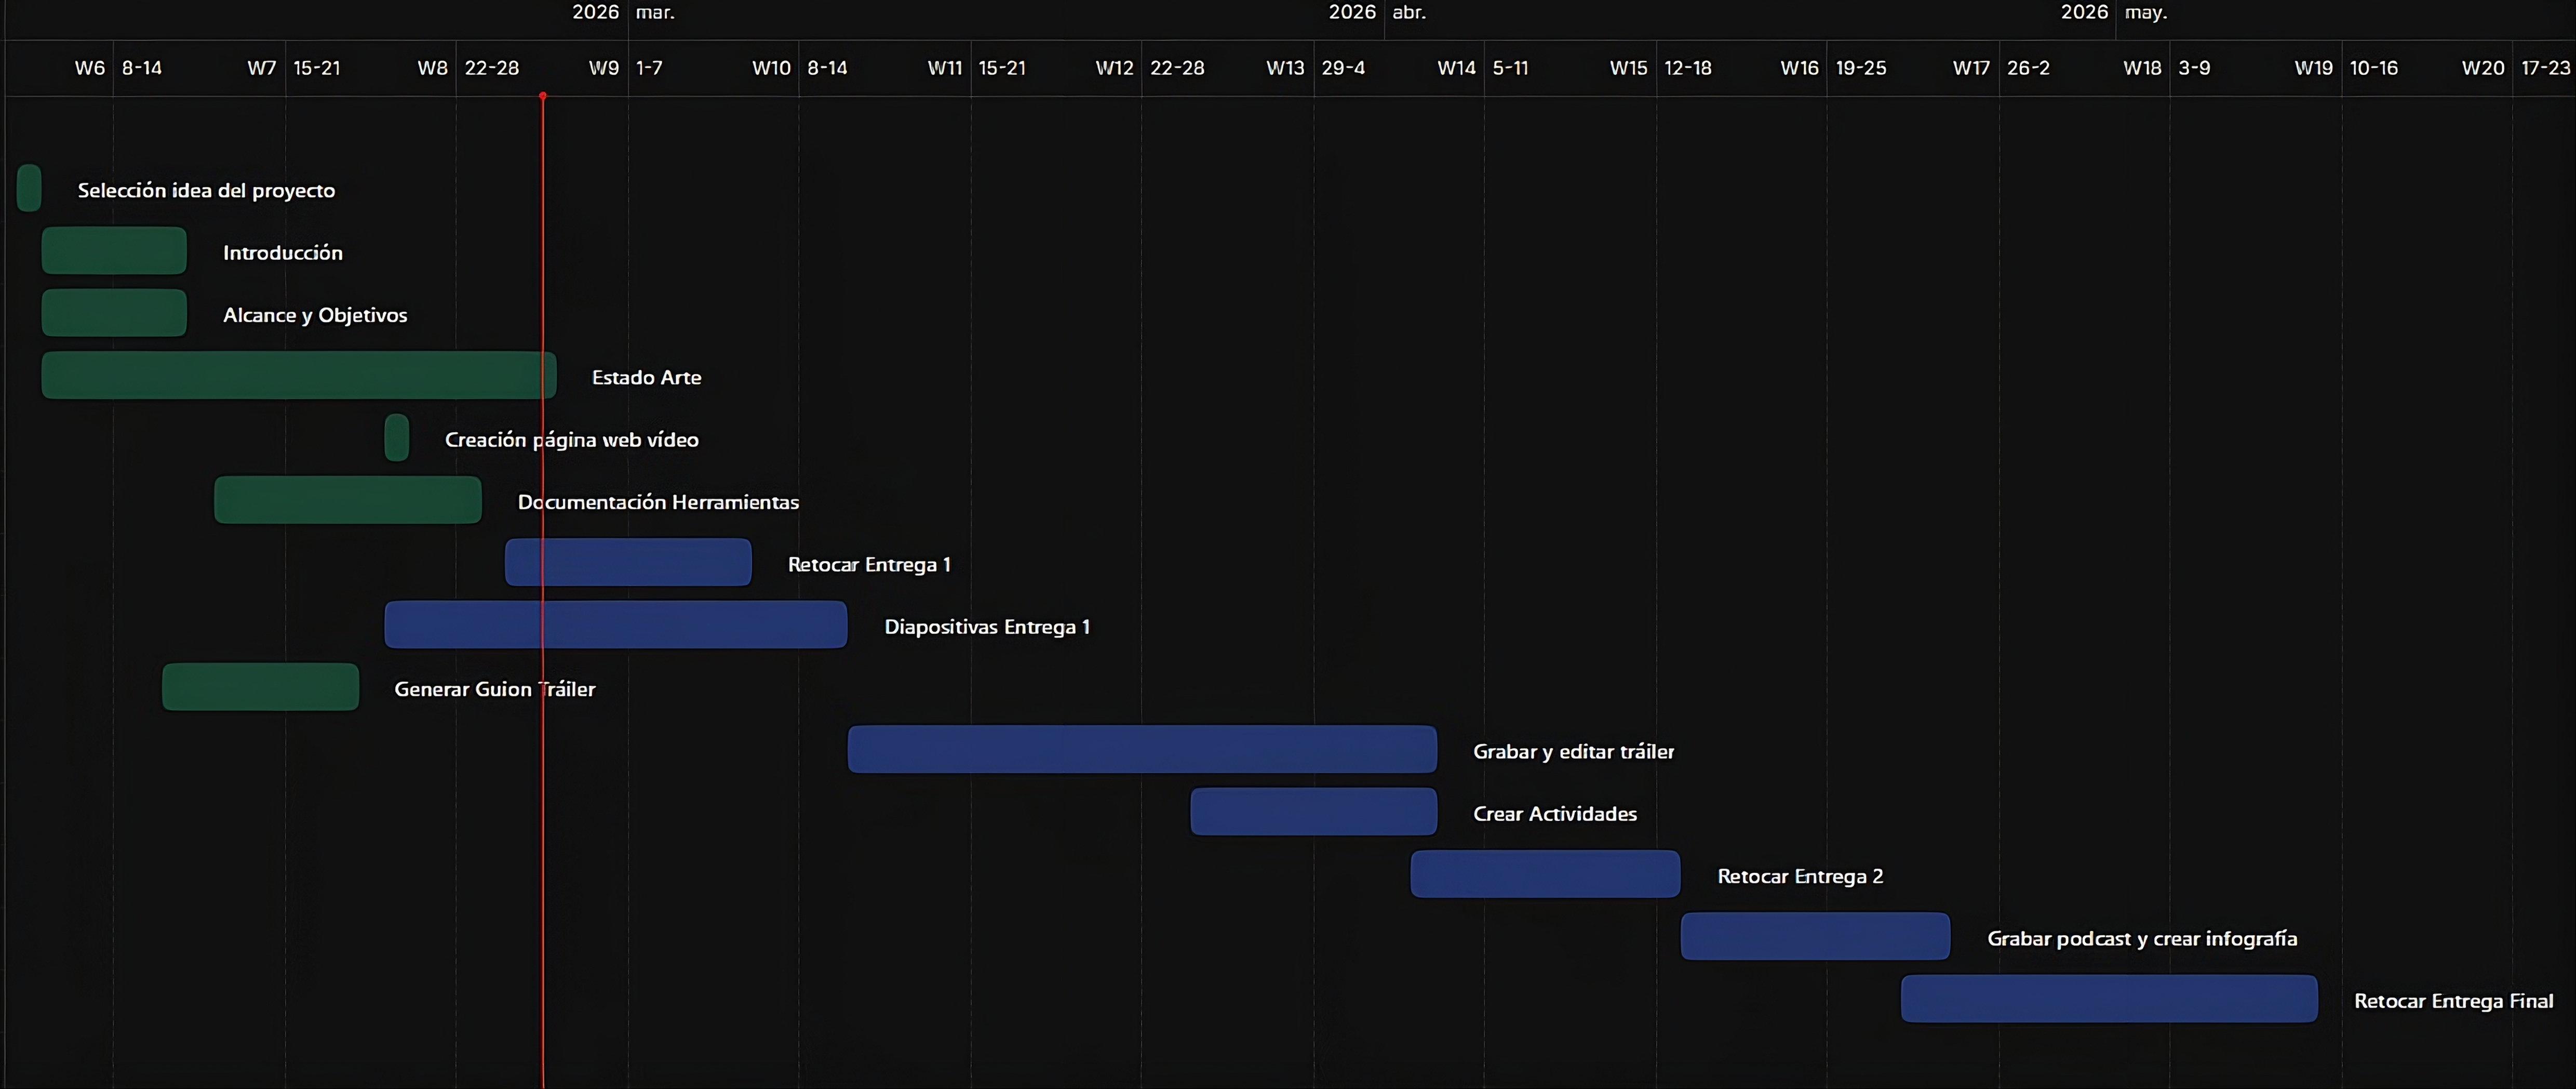
\includegraphics[width=1.\textwidth]{assets/diagrama-gantt.png}
    \caption{Representación visual \textbf{diagrama de Gantt}}
    \label{fig:diagrama-gantt}
\end{figure}
